\section{Introduction}
Frozen time-series foundation models provide point predictions and quantiles without
training a new forecasting model for every deployment stream
\citep{ansari2024chronos,das2024timesfm,ansari2025chronos2,liu2025moirai2}.
Their uncertainty estimates can still need calibration. A comparison of complete
calibration pipelines, however, combines several choices: which predictive information
enters the score, how delayed feedback updates its level, and how much history is
retained. A better interval score does not identify which choice supplied the benefit.
Nor does it establish reliable coverage in every time period or operating regime.

This paper studies three questions on fixed neural forecasts. First, how much value
does native predictive information retain after stronger residual and interval-construction
controls? Second, what does feedback adaptation add after learning rate and memory
are selected together? Third, which reliability deficits remain when interval scores
improve? We use existing calibration methods as controlled components, keeping targets,
forecast origins and reveal schedules aligned across each comparison.

The main finding is an interaction between score construction, feedback state and
calibration memory. On a protocol-locked weather panel, the issued/shared CQR score
gap remains 6.08\% after admitting zero and very small learning rates at a fixed
window, but falls to about 0.05\% with window selection. A subsequent positive-rate
analysis produces essentially the same attenuation before zero is admitted
(Figure~\ref{fig:core}). Thus the observed collapse cannot be explained solely by
selecting an exactly zero rate. Many selected positive rates are nevertheless tiny:
the result concerns how comparisons change near the rolling limit, rather than a
proof that substantive feedback mechanisms are equivalent.

A second finding separates average-score and local-reliability benefits. At one step
on weather, adaptive CQR has only about 0.36\% mean paired score improvement over
selected-window Rolling CQR, but mean local coverage error falls from 3.15 to 1.43
percentage points. Shared and issued states coincide at one step, so this is a
feedback-level benefit rather than a state-architecture benefit. All three time blocks
retain a local improvement for three of the four weather pairs; the fourth selects
the same rolling method. This supplies a concrete boundary to an interpretation
that feedback has little value merely because its long-horizon score benefit is small.

Native-band information also survives stronger construction controls. On the original
PV panel, common nonnegative projection and an asymmetric signed-residual baseline
leave a 9.56\% positive-output score benefit. Yet CQR coverage on that subset is
86.45\% at a 90\% target, and a high-forecast group observable at issue time also
under-covers. The resulting contribution is a set of conditional empirical findings
about attribution and reliability, supported by exact coverage accounting, new-source
confirmation and a forecast-based reproduction artifact.

\begin{figure}[!htbp]\centering
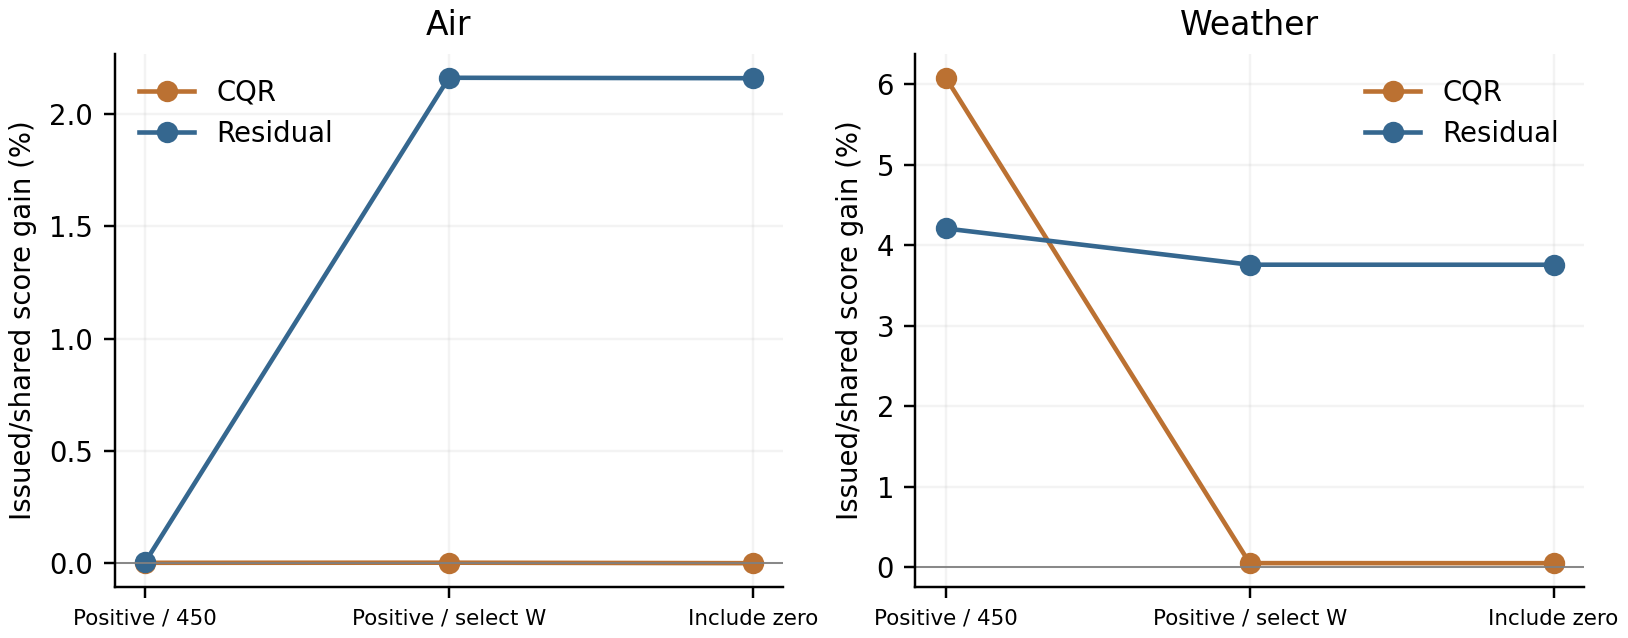
\includegraphics[width=\textwidth]{figures/positive_rates.png}
\caption{Post-review exploratory contrasts at $h=24$, four dependent pairs per
source. Positive rates include values as small as $10^{-6}$. Window selection uses
the fixed pre-test validation segment and the existing grid. The weather CQR gap
shrinks before zero is admitted; residual-score selection follows a different pattern.
These points compare selected configurations, not intrinsic state effects.}
\label{fig:core}\end{figure}

\section{Related work and comparison scope}
CQR uses predictive quantiles to define calibrated interval endpoints
\citep{romano2019cqr}; residual scaling supplies another established construction
\citep{lei2018distfree}. Online methods include ACI, adaptive aggregation, strongly
adaptive experts, PID, decaying-step optimization and optimistic updating
\citep{gibbs2021aci,zaffran2022acits,gibbs2024dtaci,bhatnagar2023saocp,
angelopoulos2023pid,angelopoulos2024decay,areces2025online,hu2026cop}.
Our primary contrasts hold the neural forecasts fixed while changing these components.
Declared implementation variants and their source checks are in \ref{app:rules}.

\citet{adler2025calibration}, published at ICLR 2026, examine native TSFM calibration,
prediction heads and rollout. Distribution-aware conformal prediction
\citep{schweizer2026dcp} already separates probabilistic predictors from scores.
We investigate a different comparison: whether changing the score changes the
apparent delayed-state benefit after rate and memory controls, and which native-band
benefits survive common support and asymmetric residual constructions. Foundation-model
conformal inference \citep{achour2025fm}, direct volatility modeling
\citep{cho2026volatility} and hidden-state-conditioned calibration
\citep{zhu2025afocp} provide related approaches; hidden representations are unavailable
in the forecast archives used here.

AcMCP models multi-step error autocorrelation and provides ACI/PID implementations
\citep{wang2026acmcp}. Its ACI uses a shared state. The delayed ACI analysis of
\citet{elhalabi2026delayed} establishes interleaving for issuing-state updates and
examines delay relative to residual memory, including rate dependence on residual
dynamics. Our window intervention changes the retained empirical score history on
the same forecast stream; it does not estimate that latent residual-memory scale.
Staggered integral control also treats delayed feedback \citep{cherenson2026staggered},
and O$^2$CP optimizes across horizons \citep{li2026o2cp}. We implement full configured
AcMCP-CSS on the complete weather subset and retain the wider PID comparison.

Three comparison types are kept distinct. Information contrasts hold the controller
fixed and change the score or interval construction. State contrasts at a fixed window
hold information and observation timing fixed, while allowing each state to select
its rate. Joint window selection compares deployable configurations; it does not
isolate state alone. AcMCP/PID versus native CQR is a complete-method comparison with
different information. These distinctions define the scope of the empirical contribution;
we do not infer new algorithmic validity guarantees from modified implementations.

\section{Causal calibration and explanatory accounting}
\subsection{Scores, observation timing and state}
At origin $t$, the frozen model emits a point forecast $m_t$ and ordered endpoints
$\ell_t,u_t$ for $y_t=Y_{t+h}$. At natural feedback lag $h$, calibration can use only
outcomes from origins $i\leq t-h$. The primary scores and inversions are
\begin{align}
s_t^{\rm R}&=|y_t-m_t|,& C_t^{\rm R}&=[m_t-q_t,m_t+q_t],\\
s_t^{\rm Q}&=\max(\ell_t-y_t,y_t-u_t),&
C_t^{\rm Q}&=[\ell_t-q_t,u_t+q_t].
\end{align}
CQR can have a negative threshold and shrink its native band. Reversed endpoints
are repaired to their midpoint and counted; coverage feedback uses the emitted
interval. Infinite scores remain infinite. The stored 0.1/0.9 band is a score input,
not an uncalibrated 90\% interval. No unrecorded tails are extrapolated. Additional
scale and midpoint controls are specified in \ref{app:details}.

Let $Q_p(\mathcal H_t)$ be the linearly interpolated empirical quantile of the last
$W$ observed, revealed scores. Rolling uses $q_t=Q_{1-\alpha}(\mathcal H_t)$, with
$\alpha=0.1$. ACI uses $q_t=Q_{1-a_t}(\mathcal H_t)$. For emitted-interval
miscoverage $e_i=\ind\{y_i\notin C_i\}$, the two established recursions are
\begin{align}
a_t^{\rm S}&=\clip_{[.001,.999]}\{a_{t-1}^{\rm S}+\gamma(\alpha-e_{t-h})\},\label{eq:shared}\\
a_t^{\rm I}&=\clip_{[.001,.999]}\{a_{t-h}^{\rm I}+\gamma(\alpha-e_{t-h})\}.\label{eq:issued}
\end{align}
They coincide at $h=1$. At larger $h$, issued updating has $h$ interleaved level
states; the common rolling history still couples their score information.
Both start at $a=\alpha$. At $\gamma=0$ they are the same Rolling method when
window and timing agree. Rolling continues to update its empirical distribution
even though it does not adjust the nominal level.

All trajectories exclude their first 600 forecast pairs from evaluation. Issuance
starts at $600+h-1$; validation uses $[600+h-1,1200-h+1)$ and testing starts at
1200, with state carried across the boundary. Thus every validation label is
available before test selection. Missing neural inputs are filled using past
observations only. Missing targets are excluded from score memory, error updates
and evaluation; issued phases continue without an increment. The full time-index
and missingness checks accompany the code.

\subsection{What the accounting explains}\label{sec:topology}
Clipping affects the usual telescoping coverage argument. For a revealed-error
update, write $r_k=a_{k+1}-a_k-\gamma(\alpha-e_k)$. Then
\begin{equation}\label{eq:identity}
\frac{1}{K}\sum_{k=1}^{K}e_k-\alpha
=\frac{a_1-a_{K+1}}{\gamma K}+\frac{\sum_{k=1}^{K}r_k}{\gamma K},\qquad\gamma>0.
\end{equation}
Bounded levels control the endpoint term but do not eliminate accumulated clipping.
For the delayed interpolation with raw update
$(1-\rho)a_{t-1}+\rho a_{t-h}+\gamma(\alpha-e_{t-h})$, define
$V_t=a_t+\rho\sum_{k=1}^{h-1}a_{t-k}$. Direct subtraction gives
\begin{equation}\label{eq:potential}
V_t-V_{t-1}=\gamma(\alpha-e_{t-h})+r_t.
\end{equation}
Shared and issued states correspond to $\rho=0,1$. The identity separates finite-time
endpoint and clipping contributions; unrevealed final outcomes are counted separately.
It is not a proof of conditional validity or a decomposition of all score differences.

Under a stationary differentiable miscoverage response with slope $g>0$, inactive
clipping and deterministic response feedback, linearized shared and issued errors
satisfy $x_t=x_{t-1}-\gamma g x_{t-h}$ and $x_t=(1-\gamma g)x_{t-h}$.
Their familiar stability ranges are
\begin{equation}\label{eq:stability}
0<\gamma g<2\sin\!\left(\frac{\pi}{4h-2}\right)\quad(\mathrm{shared}),
\qquad 0<\gamma g<2\quad(\mathrm{issued}).
\end{equation}
The first is the classical scalar delay-difference boundary
\citep{deger2017stability}; issued contraction per calendar step is
$|1-\gamma g|^{1/h}$. A wider stable gain range therefore need not mean faster
tracking. These approximations motivate rate controls. Empirical quantile jumps,
changing memory and clipping require the actual trajectory diagnostics in \ref{app:rates}.

\section{Experimental design}
\subsection{Evidence panels and analysis stages}
The original main panel has 31 series and four archived backbones (Chronos-2,
Chronos-Bolt, TimesFM and Moirai): 25 observed energy series, four constructed
series and two synthetic switches. Separate renewable and multi-horizon archives
provide supporting diagnostics. An original confirmation uses traffic and exchange
rates with two Chronos models, giving 16 pairs per horizon. These sources, time
units and archive limitations are specified in \ref{app:data}.

A further locally fixed protocol precedes numeric acquisition of two new sources:
Jena roof temperature and pressure in the first 3,600 hours of 2026, and PM2.5 at
two Beijing stations in the first 3,600 hours from 1 March 2013
\citep{jena2026weather,chen2017air}. The same two cached Chronos checkpoints generate
24 horizons at 2,976 consecutive origins, with context 512. Each test has 1,776
origins before excluding missing targets. Weather forecast targets are complete;
air-quality masks are retained. Four series and two models yield eight dependent
pairs, not eight independent replications.

Original and new-source confirmation choices were recorded before their respective
acquisitions. Later rate sensitivities, PV controls and the present positive-rate,
time-block and history analyses revisit inspected data and are exploratory.
Local timestamp/hash records are not external preregistration. Neither source novelty
within this calibration project nor recent observation dates establish exclusion
from neural pretraining. Detailed grids and chronology are in \ref{app:newprotocol}.

\subsection{Selection and comparisons}
The original matched ACI comparison selects each score's $(\gamma,W)$ from three
rates and $W\in\{200,450,900\}$. The new-source protocol nests the original three
rates, a wider grid with delay-scaled values, zero/small rates down to $10^{-6}$,
and finally window selection. Each state minimizes its own validation interval
score, with ties favoring smaller rate and then window. A separately selected
zero-rate Rolling control uses the same candidate windows. Test scores never
choose the search range. Positive-rate reanalysis uses only existing candidates,
holding $W$ fixed or selecting it before finally admitting zero.

Full AcMCP-CSS uses the pinned author's MA$(h-1)$ and cross-horizon regression,
all 24 horizons, history 600, and validation-selected learning rates. CSS is the
author's supported fitting option; its estimates need not equal default CSS-ML.
We add history 450 for a bounded sensitivity. Because the author's history parameter
also governs startup, this additional comparison uses a common post-startup
validation block $[900+h-1,1200-h+1)$, unchanged tests, and common histories
$\{450,600\}$ for CQR, Rolling and AcMCP/PID. Every evaluated scorecast is checked
finite. Fixed-600 and selected-history results answer complementary fairness
questions without presenting different fitting windows as equivalent algorithms.

On all 32 original PV pairs, the signed-error comparator uses
$[m_t+Q_{a_t/2}(Y-m),m_t+Q_{1-a_t/2}(Y-m)]$ with the same total-miscoverage state.
Each construction is tuned before and after common support projection
$[L,U]\mapsto[\max(0,L),\max(0,U)]$. Projection leaves each candidate's raw feedback
trajectory unchanged, isolating emitted-interval geometry. For a nonnegative target
it cannot increase interval score or lose a covered observation. In addition to
actual zero/positive groups, an issue-time grouping uses whether $m_t$ exceeds
the median of the first 600 forecasts. Its threshold never uses test outcomes.

\subsection{Metrics and temporal resolution}
For $[L,U]$, we use the proper interval score
\begin{equation}
\IS_\alpha=(U-L)+\frac{2}{\alpha}(L-y)_++\frac{2}{\alpha}(y-U)_+,
\end{equation}
alongside coverage and local absolute coverage error over 150-origin windows
\citep{winkler1972,gneiting2007proper}. Missing targets are excluded from each
window's denominator. Paired score gain is $100(1-\IS_A/\IS_B)$; ratios and gains
are calculated within each model--series pair before averaging, with equal source
weight for equal-sized confirmation panels. A positive local-error improvement
means the comparator's error minus the candidate's, in percentage points.

Three consecutive 592-origin test blocks reveal temporal heterogeneity without
reselecting models. Block-local windows stay within each block. The main-panel
bootstrap and dependence checks remain in the supplementary records; confirmation
pair counts and tiny score differences are descriptive, not independent-replication
confidence statements. We report score, overall coverage and local error together.

\section{Results}
\subsection{RQ1: What predictive-information benefits survive stronger controls?}
Across 124 main-panel pairs, default CQR--ACI improves score by 13.57\% relative
to default symmetric residual--ACI. Tuning both methods reduces the paired benefit
to 9.98\%. The latter is recomputed from every prediction archive and all nine
candidate settings for each score. Native-scale and midpoint controls, the full
original method table and family heterogeneity remain in \ref{app:details} and
\ref{app:earlierdiagnostics}; the default CQR benefit is 6.03\% after excluding PV.
On traffic/exchange rates, holding COP fixed gives native-score benefits of
12.27\%, 14.66\% and 22.16\% at $h=1,6,24$, respectively. Magnitudes depend on the
controller and panel; the comparisons do not pool scores in incompatible units.

The PV controls test two simpler explanations for the large original solar result:
symmetric intervals and extension into impossible negative outputs. Table~\ref{tab:pvcontrols}
shows that the positive-output benefit declines from 12.77\% to 11.57\% after
common projection, and to 9.56\% against projected signed residuals. Native information
therefore retains value after both controls. Successive percentages have different
denominators and selected settings, so their differences are not additive causal
contributions. The original zero/positive score decomposition and all width and
miss-penalty terms remain in \ref{app:solarparts} and \ref{app:details}.

\begin{table}[!htbp]\centering\scriptsize
\caption{PV construction controls, all 32 pairs, validation-tuned. Gains are mean
paired CQR improvements over the named baseline (\%); coverages are percent.
High forecast is an issue-time observable prefix-median split.}
\label{tab:pvcontrols}\begin{tabular}{lllrrr}
\toprule
Support & Baseline & Group & CQR gain & Cov. CQR & Cov. base \\
\midrule
Raw & Residual & all & 20.51 & 89.72 & 89.34 \\
Raw & Residual & positive & 12.77 & 86.32 & 80.17 \\
Raw & Residual & forecast high & 14.70 & 87.03 & 82.91 \\
Nonnegative & Residual & all & 15.61 & 91.56 & 90.55 \\
Nonnegative & Residual & positive & 11.57 & 86.45 & 80.50 \\
Nonnegative & Residual & forecast high & 12.41 & 87.07 & 83.04 \\
Nonnegative & Signed & all & 10.86 & 91.56 & 91.40 \\
Nonnegative & Signed & positive & 9.56 & 86.45 & 80.09 \\
Nonnegative & Signed & forecast high & 9.26 & 87.07 & 84.59 \\
\bottomrule
\end{tabular}
\end{table}

\subsection{RQ2: What does adaptation add after rate and memory selection?}\label{sec:rates}
The earlier traffic/exchange-rate sensitivity reduced the CQR issued/shared gain
at $h=24$ from 8.43\% to 0.99\% after widening the rate range. On the new-source
confirmation, small/zero rates remove the air-quality gap but leave 6.08\% on
weather at $W=450$. Adding window selection lowers that gap to about 0.05\%
(Table~\ref{tab:newconfirm}). This is why a rate-only explanation is incomplete.

\begin{table}[!htbp]\centering\small
\caption{Locked new-source confirmation at $h=24$. Mean paired issued/shared
score gain (\%), four pairs per source. Only the last column selects memory.}
\label{tab:newconfirm}\begin{tabular}{llrrrr}
\toprule
Source & Score & Original & Wide & Zero/small & Window \\
\midrule
Air quality & Residual & 15.04 & 3.08 & 0.00 & 2.16 \\
Air quality & CQR & 10.59 & 0.23 & 0.00 & 0.00 \\
Weather & Residual & 7.82 & 4.32 & 4.21 & 3.76 \\
Weather & CQR & 9.21 & 6.11 & 6.08 & 0.05 \\
\bottomrule
\end{tabular}
\end{table}

Does this attenuation merely select the identical zero-rate method? The post-review
positive-rate controls separate those possibilities (Table~\ref{tab:positive}).
Weather CQR has a 6.080\% gap with positive rates at $W=450$, 0.052\% when
positive-rate methods select their window, and 0.052\% after zero is admitted
at the displayed precision. The window-dependent attenuation therefore occurs
without exact zero. However, six of eight issued and seven of eight shared CQR
positive-rate selections use $10^{-6}$; positivity alone does not establish
substantial feedback. The result describes the tested search and its rolling limit.

\begin{table}[!htbp]\centering\small
\caption{Exploratory positive-rate decomposition, $h=24$, mean paired state gain
(\%). The first three columns exclude zero. ``Select $W$'' uses 200, 450 and 900;
``Add zero'' differs only by admitting zero. Tiny rates remain eligible.}
\label{tab:positive}\begin{tabular}{llrrrr}
\toprule
Source & Score & $W=450$ & $W=900$ & Select $W$ & Add zero \\
\midrule
Air & CQR & 0.002 & -0.003 & 0.002 & 0.000 \\
Air & Residual & 0.004 & 2.161 & 2.161 & 2.159 \\
Weather & CQR & 6.080 & 0.052 & 0.052 & 0.052 \\
Weather & Residual & 4.208 & 0.001 & 3.759 & 3.758 \\
\bottomrule
\end{tabular}
\end{table}

Residual scores show why selected configurations must also be inspected. On weather,
their state gap is essentially zero when both use $W=900$, yet is 3.759\% after
independent window selection. The shared residual method selects $W=450$ for both
pressure series while the issued method selects 900. The resulting test gap is
partly a difference in validation-selected memory, not a residual intrinsic state
effect. On air quality, allowing window selection also brings back a residual gap.
Larger validation searches need not improve every test result.

Table~\ref{tab:choices} exposes every final CQR choice. Six of eight pairs choose
the exact same zero-rate/window method. The two pressure pairs choose distinct
settings and retain small score differences. Seven of eight configurations in each
state select the largest allowed window; early and late validation select identical
settings for only three issued and four shared pairs. These boundary and stability
checks preclude interpreting the final mean as a precisely identified state effect.

\begin{table}[!htbp]\centering\scriptsize
\caption{Every final CQR pair at $h=24$, original full-validation selector. S/I
are shared/issued; C2 and Bolt are the two Chronos models. IS is in the respective
series' units. Same rolling means both rates are zero with the same window.
Air A/D denote Aotizhongxin/Dingling.}
\label{tab:choices}\begin{tabular}{lrrrrrrl}
\toprule
Pair & $\gamma_S$ & $W_S$ & IS$_S$ & $\gamma_I$ & $W_I$ & IS$_I$ & Selection \\
\midrule
Air A / C2 & 0 & 900 & 288.250 & 0 & 900 & 288.250 & Same rolling \\
Air A / Bolt & 0 & 450 & 319.915 & 0 & 450 & 319.915 & Same rolling \\
Air D / C2 & 0 & 900 & 238.382 & 0 & 900 & 238.382 & Same rolling \\
Air D / Bolt & 0 & 900 & 300.438 & 0 & 900 & 300.438 & Same rolling \\
Pressure / C2 & 0.0001 & 900 & 21.442 & 0.002 & 900 & 21.437 & Distinct \\
Pressure / Bolt & 0 & 900 & 20.385 & 0.00208 & 900 & 20.348 & Distinct \\
Temperature / C2 & 0 & 900 & 15.152 & 0 & 900 & 15.152 & Same rolling \\
Temperature / Bolt & 0 & 900 & 14.491 & 0 & 900 & 14.491 & Same rolling \\
\bottomrule
\end{tabular}
\end{table}

Against separately window-selected Rolling CQR, the final issued CQR mean score
gain is zero on air quality and 0.04\% on weather at $h=24$; weather coverage is
89.43\% versus 89.51\%. The earlier traffic/exchange-rate comparison likewise
gives only 0.17\% mean gain over Rolling. COP instead has a 2.90\% higher score
there but better overall and local coverage. The correct interpretation requires
the reliability comparisons in RQ3, rather than a score-only ranking.

\paragraph{A common-history AcMCP check.}
The original full AcMCP-CSS comparison used history 600 against CQR allowed to
select 200/450/900. At $h=24$ its mean paired score ratio to selected Rolling was
1.147, with 87.54\% coverage. The extra comparison in Table~\ref{tab:history}
restricts all methods to common history options and a common post-startup validation
segment. It includes every weather pair and the no-scorecast PID ablation.
With common history 600, AcMCP's score ratio is 1.172; selecting 450/600 gives
1.164, with 89.18\% coverage. Fixed 450 scores better on the test than the joint
selector, another reminder that validation search is not a test oracle. Issued
CQR remains close to Rolling, whereas shared CQR has a 1.039 score ratio under
the joint selector. Thus the nearly zero original state gap does not persist
under every history and validation choice.
The history check is a bounded complete-configuration sensitivity; native CQR and
signed-error methods still receive different predictive information. All horizons,
selected rates, success counts and source checks are retained in \ref{app:focused}.

\begin{table}[!htbp]\centering\small
\caption{Common-history weather comparison at $h=24$, four pairs. All rows use
the same post-startup validation block and unchanged test origins. Each IS ratio
uses its matched Rolling method within that history search; coverage is percent
and Local is percentage points.}
\label{tab:history}\begin{tabular}{llrrr}
\toprule
History & Method & IS ratio & Coverage & Local \\
\midrule
450 & Rolling-CQR & 1.000 & 89.32 & 6.33 \\
450 & CQR-shared & 1.136 & 83.22 & 8.96 \\
450 & CQR-issued & 1.000 & 89.27 & 6.34 \\
450 & AcMCP-CSS & 1.138 & 89.18 & 6.45 \\
450 & PID-no-scorecast & 1.061 & 88.20 & 6.49 \\
600 & Rolling-CQR & 1.000 & 89.44 & 6.75 \\
600 & CQR-shared & 1.039 & 87.43 & 7.42 \\
600 & CQR-issued & 1.000 & 89.43 & 6.74 \\
600 & AcMCP-CSS & 1.172 & 89.27 & 6.27 \\
600 & PID-no-scorecast & 1.067 & 88.37 & 6.43 \\
450/600 & Rolling-CQR & 1.000 & 89.44 & 6.75 \\
450/600 & CQR-shared & 1.039 & 87.43 & 7.42 \\
450/600 & CQR-issued & 1.000 & 89.43 & 6.74 \\
450/600 & AcMCP-CSS & 1.164 & 89.18 & 6.48 \\
450/600 & PID-no-scorecast & 1.065 & 88.60 & 6.24 \\
\bottomrule
\end{tabular}

\end{table}

\subsection{RQ3: Which reliability gains and deficits remain?}\label{sec:rolling}
Adaptive levels can supply local reliability even when average-score improvements
are small. On weather at $h=1$, adaptive CQR improves mean paired score by 0.36\%
while reducing average local coverage error from 3.15 to 1.43 percentage points.
Table~\ref{tab:localpairs} shows every pair and every test block. Both pressure
series and Chronos-2 temperature improve local error in all three blocks, despite
mixed signs for their score gains. Chronos-Bolt temperature selects the same
zero-rate rolling configuration and has identical results. This is neither a
universal benefit nor an effect of issued versus shared states, which coincide
at one step.

\begin{table}[!htbp]\centering\scriptsize
\caption{Weather $h=1$: adaptive CQR versus selected-window Rolling. Gain is
paired score improvement (\%). Whole-test local errors and their block improvements
are percentage points; positive block values favor ACI. All configurations are
selected before testing.}
\label{tab:localpairs}\begin{tabular}{lrrrrrr}
\toprule
Pair & Score gain & Local roll & Local ACI & Early & Middle & Late \\
\midrule
Pressure / C2 & +1.77 & 4.51 & 1.45 & +2.83 & +3.88 & +3.81 \\
Pressure / Bolt & +0.20 & 3.75 & 0.86 & +2.76 & +2.58 & +3.01 \\
Temperature / C2 & -0.54 & 2.14 & 1.19 & +1.08 & +1.05 & +1.15 \\
Temperature / Bolt & +0.00 & 2.21 & 2.21 & +0.00 & +0.00 & +0.00 \\
\bottomrule
\end{tabular}
\end{table}

The benefit varies with horizon and source (Table~\ref{tab:tradeoff}). The complete
block-by-pair display in \ref{app:focused} shows where favorable averages conceal
different time periods. These descriptive slices identify the empirical extent
of the benefit; they do not establish that a measured drift variable caused it.
The average interval score rewards width and miss distance, whereas local coverage
error penalizes persistent deviations from the target frequency. Improvements on
one metric therefore need not have the same size or sign on the other.

The same distinction is visible for another method. In the common-history
sensitivity at $h=1$ and history 600, AcMCP-CSS has a score ratio of 1.023 but
local error of 2.09 percentage points, compared with Rolling's 3.44. PID reaches
1.86 points. These use the same later validation block and fixed history, so
their local gains are not compared with a differently tuned Rolling denominator.
Local-reliability value is therefore not exclusive to native CQR, and a slightly
worse average score need not make a feedback configuration uniformly inferior.

\begin{table}[!htbp]\centering\scriptsize
\caption{Whole-test tradeoffs for the original new-source selector, four pairs
per source. ACI denotes issued CQR (identical to shared at $h=1$); gain is relative
to selected-window Rolling CQR. Coverage is percent and Local is percentage points.}
\label{tab:tradeoff}\begin{tabular}{lrrrrrr}
\toprule
Source & $h$ & Gain & Cov. roll & Cov. ACI & Local roll & Local ACI \\
\midrule
Air & 1 & -0.77 & 90.59 & 90.55 & 2.32 & 1.94 \\
Air & 6 & +0.00 & 89.65 & 89.65 & 4.85 & 4.85 \\
Air & 24 & +0.00 & 89.84 & 89.84 & 6.37 & 6.37 \\
Weather & 1 & +0.36 & 89.37 & 89.44 & 3.15 & 1.43 \\
Weather & 6 & -0.18 & 90.27 & 90.44 & 2.91 & 2.91 \\
Weather & 24 & +0.04 & 89.51 & 89.43 & 6.03 & 6.01 \\
\bottomrule
\end{tabular}
\end{table}

Exact clipping accounting explains one concrete coverage cost in the older
traffic/exchange-rate panel. Original-grid shared CQR has 2.150 percentage points
of revealed-test excess miscoverage: 2.117 from clipping and 0.033 from the endpoint
term. With scaled rates, clipping falls to 0.336 while the endpoint term rises to
0.681. Smaller rates suppress one cost while increasing a finite-time adaptation
term. The full identity and controlled stability/tracking simulations are in
\ref{app:rates}; this accounting does not assign every score change to instability.

PV exposes a different reliability deficit. Under the strongest construction
control in Table~\ref{tab:pvcontrols}, CQR covers 91.56\% overall but only 86.45\%
of positive targets. The issue-time high-forecast group has a 9.26\% score gain
against projected signed residuals, yet only 87.07\% coverage. Projection can
newly cover zero outputs when both raw endpoints were negative, improving overall
coverage without resolving positive-output reliability. Thus the retained native
information benefit and the retained operational gap are simultaneous findings.

\section{Discussion and limitations}
The evidence supports a sequence of evaluation decisions. Establish native-information
value under matched controllers and plausible interval geometry. Then compare
feedback updates with selected-window Rolling, separating a common-window state
contrast from a joint configuration-selection contrast. Finally inspect local and
observable-group reliability. This sequence distinguishes three outcomes observed
here: surviving native-band benefits, a window-sensitive state-score difference
that becomes practically small, and local benefits that average scores understate.

The zero-rate result has a precise interpretation. Six pairs select the same
method, so equality is mathematically expected; the empirical finding is that
validation chooses that method and it remains competitive on later observations.
The positive-only controls show that exact degeneracy is not the sole explanation
for the weather attenuation, but tiny selected rates and window boundaries remain
important. The residual fixed-window versus selected-window contrast further
shows how a favorable apparent state gap can arise from different memory choices.
These observations guide fair comparisons without providing a universal controller
selection rule.

Generality remains limited. Weather comes from one site and two variables; air
quality uses two correlated stations, with two models and relatively short tests.
The panels include dependent energy series and constructed switches. New-source
choices were locked locally, whereas the positive-only, block and extra history
analyses use inspected data. All selectors and negative results are retained, but
these sensitivities are not additional independent confirmations. Broader uninspected
deployments would be needed to validate a practical adaptation-selection rule.

Finite search boundaries also matter. Maximum-window selections are frequent, and
the extra AcMCP comparison covers histories 450/600 with CSS and a fixed integrator
configuration. It does not optimize every AcMCP setting or implement O$^2$CP.
Complete-method rankings cannot isolate controller quality. Original historical
checkpoint metadata remain incomplete; exact spot checks and paired forecasts
support the calibration comparison but do not prove training-data exclusion.
The new archives retain checkpoint hashes and generation details. The default
CPU artifact reruns calibration; optional R fitting and neural generation have
separate dependencies and declared scope.

Finally, overall or local frequency diagnostics do not establish conditional coverage,
and lower interval score does not by itself quantify operational savings. The latter
would require a decision policy and explicit shortfall costs. Our contribution is
the tested attribution and reliability evidence at the stated scales, with those
boundaries visible rather than absorbed into a single method ranking.

\section{Conclusion}
Native predictive information retains benefits after matched tuning, support and
asymmetric-residual controls. Delayed-state score advantages depend on rate and
memory selection; the weather gap shrinks under positive-rate window controls
before exact zero is admitted. Near-rolling long-horizon scores coexist with
one-step local-reliability benefits from adaptive levels, while PV subgroup
undercoverage persists. Reporting these distinctions changes how calibration
methods should be compared and how their deployment evidence should be interpreted.

\section*{Data and code availability}
Supplementary Software S1 (\texttt{Supplementary\_Software\_S1.zip}) contains
164 forecast archives, source/protocol hashes, CPU reproduction, reference results
and an explicit \texttt{ARTIFACT\_MAP.md}. The entry point recomputes the 124-pair
headline, rate/window searches, PV controls and the new focused analyses. Cached
AcMCP replay uses supplied R fits; separate commands refit the full author algorithm.
Earlier unrerun controllers remain identified historical inputs. A repository URL
will be added after author upload; the prepared archive is the reviewer-access package.

\section*{Funding}
This work is supported by the National Natural Science Foundation of China
(Grant No. 62372409).
\section*{Declaration of competing interest}
The authors declare no competing interests.
\section*{Declaration of generative AI and AI-assisted technologies}
OpenAI Codex assisted with literature retrieval, code auditing, experiment implementation,
analysis and manuscript preparation. The authors remain responsible for reviewing the
methods, results, citations and final text.
